\chapter{Demo Application}

A custom printed circuit board (PCB) was created for this thesis. The board was used for real world power measurements of different sensor data acquisition techniques, and to show some potential IoT applications. 

\section{Demo Board}

\subsection{nRF51}

The nRF51 is a Cortex-M0+ based System-on-Chip (SoC) from Nordic Semiconductor. The company is world leading in creating Bluetooth Low Energy solutions. This SoC was chosen mainly because of its advanced power saving features. 

The nRF51 features several serial interfaces. However, only the SPI module has DMA capabilities. It is therefore necessary to choose an accelerometer with an SPI interface. This only rules out the MMA8491QR1 from Freescale Semiconductor.

For optimal power efficiency it is optimal to use the lowest possible supply voltage. The nRF51822 can go as low as 1.8V.

\begin{center}
    \begin{tabular}{| l |}
    \hline
    6.3mA - TX at -4dBm (3V using on-chip DC-DC) \\ \hline
    8.0mA - TX at 0dBm (3V using on-chip DC-DC) \\ \hline
    11.8mA – TX at +4dBm (3V using on-chip DC-DC) \\ \hline
    9.7mA – RX (3V using on-chip DC-DC) \\ \hline
    13mA – RX at 1Mbps (No DC-DC) \\ \hline
    10.5mA – TX at 0dBm (No DC-DC) \\ \hline
    0.6µA – SYSTEM-OFF, no RAM retention \\ \hline
    1.2µA - SYSTEM-OFF, 8KB RAM retention \\ \hline
    2.6µA - SYSTEM-ON, All peripherals in idle mode \\ \hline
    \end{tabular}
\end{center}

\subsubsection{Programmable Peripheral Interconnect (PPI)}

The nRF51 features something the company calls Programmable Peripheral Interconnect (PPI). The PPI enables different peripherals in the device to interact autonomously with each other using tasks and events without using the CPU. The PPI can automatically trigger a task in one peripheral as a result of an event occurring in another. For instance, an interrupt from an external device (i.e. accelerometer) can trigger the SPI module to initiate a block transfer to memory. 

\subsubsection{EasyDMA}

The EasyDMA function in the nRF51 is able to move data to and from RAM and autonomously between peripherals. The DMA can be configured to work in conjunction with the PPI system for fully autonomous operation.

So in turn one should be able to make a sensor data acquisition system that is able to collect accelerometer data and send it over radio without using the CPU.

\subsubsection{GPIOTE}

\subsubsection{Bluetooth Low Energy}

Bluetooth Low Energy (BLE) is wireless communication protocol designed by the Bluetooth Special Interest Group. The protocol is aimed at healthcare, fitness and beacon applications. It is designed to have ultra-low peak, average and idle mode power consumption. This enables devices that uses BLE to run for years on a standard coin-cell battery. BLE has become a big part of IoT applications that are available today, and is considered to be an important protocol for future devices as well. Another benefit with BLE, is that most smart phones support the protocol and are therefore able to talk to other BLE devices. Low-power and connectivity was the main reason that BLE was chosen for this demo application. 

\section{The Configuration}

The planned example will utilize EasyDMA, PPI, GPIOTE, SPI and the radio of the nRF51, as viewed with red boxes in Figure \ref{fig:accel_working_principle}. The Cortex-M0+ CPU should only be used for configuration of the system, and will be sleeping during data collection. The ADXL362 is configured to wake up when motion is detected, and then collect samples autonomously into its embedded FIFO. When the FIFO is full, the ADXL362 will send an interrupt to nRF51. The PPI is configured to listen to for this interrupt and to trigger a SPI block transfer when it is detected. As data is being transferred to the SPI module, the EasyDMA shuffles data either into the RAM or the radio module. This entire operation is possible without any CPU intervention.

\begin{figure}[h]
\centering
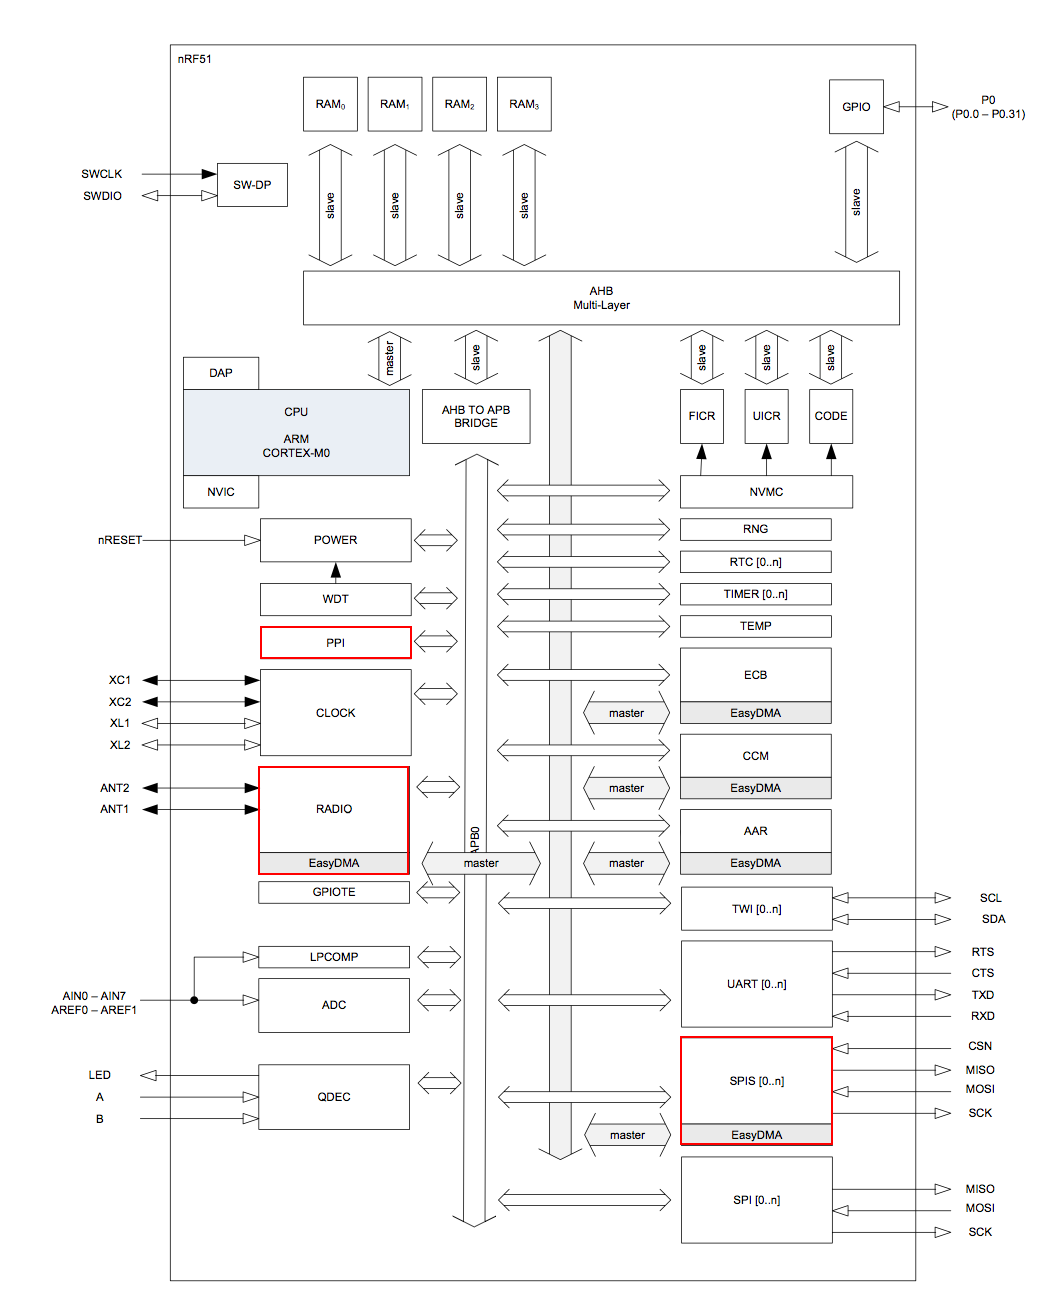
\includegraphics[scale=0.5]{fig/nrf51822_edit.png}
\caption{Nordic nRF51 System architecture. \cite{nRF51}}
\label{fig:accel_working_principle}
\end{figure}

\subsection{Power Estimation}

\begin{itemize}
\item Run current for SPI @ 4Mbps = 200$\si{\micro\ampere}$
\item Run current for GPIOTE (port event) = < 1$\si{\micro\ampere}$
\end{itemize}

Listen state:
\begin{equation}
I_{total} = \text{nRF51 (SYSTEM-OFF, 8KB RAM rentention)} + \text{GPIOTE} + \text{ADXL362 (Wake-up mode)}
\end{equation}

\begin{equation}
I_{total} = 1.2\si{\micro\ampere} + 0.1\si{\micro\ampere} + 0.27\si{\micro\ampere} = 1.57\si{\micro\ampere} 
\end{equation}

Motion state:

\begin{equation}
I_{total} = \text{nRF51 (SYSTEM-OFF, 8KB RAM rentention)} + \text{GPIOTE} + \text{SPI (4Mbps)} + \text{ADXL362 (400Hz ODR)}
\end{equation}

\begin{equation}
I_{total} = 1.2\si{\micro\ampere} + 0.1\si{\micro\ampere} + 200\si{\micro\ampere} + 3.0 \si{\micro\ampere} = 204.3\si{\micro\ampere} 
\end{equation}